\documentclass[12pt, a4paper, bahasa]{article}

\usepackage[margin=2.5cm]{geometry}
\usepackage{fancyhdr}
\PassOptionsToPackage{hyphens}{url}
\usepackage{hyperref}
\usepackage{graphicx}
\usepackage{float}
\usepackage{titlesec}
\usepackage{wrapfig}
\usepackage{subcaption}
\usepackage{csquotes}
\usepackage{amsmath}
\usepackage{amssymb}
\usepackage{listings}
\usepackage{xcolor}

% Pengaturan Header dan Footer
\pagestyle{fancy}
\setlength{\headheight}{14.5pt}
\fancyfoot[C]{\thepage}
\lhead{\textbf{Nama:} Khalilullah Al Faath}
\rhead{\textbf{NIM:} 25/566643/PPA/07139}
\renewcommand{\headrulewidth}{0.4pt}
\renewcommand{\footrulewidth}{0.4pt}

\renewcommand{\tablename}{Tabel}
\renewcommand{\figurename}{Gambar}

% Pengaturan listing kode
\lstset{
    basicstyle=\ttfamily\small,
    frame=single,
    breaklines=true,
    keepspaces=true,
    columns=fullflexible,
    morecomment=[l]{\#},
    commentstyle=\color{red},
    belowskip=0pt,
    showstringspaces=false
}

\pagenumbering{arabic}
\begin{document}

\begin{center}
    \large \textbf{Theory of Computation -- Assignment 4} \\[0.2cm]
    \large Encoding \\[0.5cm]
\end{center}

% =========================================================
% PROBLEM 4.1
% =========================================================

\section{Problem 4.1 -- Injektivitas Fungsi Pemasangan Cantor}

Fungsi pemasangan Cantor $\pi:\mathbb{N}^2\to\mathbb{N}$ didefinisikan
$$\pi(a,b) = \tfrac{1}{2}(a+b)(a+b+1) + b.$$
Akan dibuktikan bahwa $\pi$ injektif, yaitu $\pi(a_1,b_1)=\pi(a_2,b_2)
\implies (a_1,b_1)=(a_2,b_2)$.

\textbf{Bukti.} Misalkan $\pi(a_1,b_1)=\pi(a_2,b_2)$. Tulis $s_1=a_1+b_1$
dan $s_2=a_2+b_2$, serta definisikan bilangan segitiga
$T(s)=\tfrac{1}{2}s(s+1)$ (sehingga $\pi(a,b)=T(a+b)+b$).

\textit{Langkah 1: $s_1=s_2$.} Untuk $a+b=s$ tetap dengan $a,b\geq0$, nilai
$b$ berkisar $0\leq b\leq s$, sehingga $\pi(a,b)=T(s)+b$ berkisar pada
interval $[T(s),\,T(s)+s]$. Karena $T(s+1)=T(s)+s+1$, interval ini sama
dengan $[T(s),\,T(s{+}1)-1]$. Andaikan $s_1\neq s_2$; tanpa mengurangi
keumuman misalkan $s_1<s_2$, sehingga $s_1+1\leq s_2$. Karena $T$ naik
tegas (monoton), $T(s_1{+}1)\leq T(s_2)$. Akibatnya
\begin{align*}
\pi(a_1,b_1) &= T(s_1)+b_1 \leq T(s_1)+s_1 = T(s_1{+}1)-1 \\
             &\leq T(s_2)-1 < T(s_2) \leq T(s_2)+b_2 = \pi(a_2,b_2),
\end{align*}
yang kontradiksi dengan $\pi(a_1,b_1)=\pi(a_2,b_2)$. Jadi $s_1<s_2$
mustahil; dengan argumen simetris $s_2<s_1$ juga mustahil. Maka $s_1=s_2$,
sebut $s$.

\textit{Langkah 2: $(a_1,b_1)=(a_2,b_2)$.} Dengan $s_1=s_2=s$, persamaan
awal menjadi $T(s)+b_1=T(s)+b_2$, sehingga $b_1=b_2$. Karena
$a_1=s-b_1=s-b_2=a_2$ (memakai $a_1+b_1=a_2+b_2=s$), diperoleh pula
$a_1=a_2$.

Jadi $(a_1,b_1)=(a_2,b_2)$, yang membuktikan $\pi$ injektif. $\blacksquare$

% =========================================================
% PROBLEM 4.2
% =========================================================

\section{Problem 4.2 -- \textit{replace} adalah WHILE-Computable}

\subsection{Definisi Ulang Masalah}
Untuk list $a=(a_1,\dots,a_n)\in\mathbb{N}^*$ dengan $enc(a)=x_1$, jika
$1\leq x_2\leq n$ maka
$$replace(x_1,x_2,x_3)=enc\big((a_1,\dots,a_{x_2-1},\,x_3,\,a_{x_2+1},\dots,a_n)\big),$$
dan $replace(x_1,x_2,x_3)\uparrow$ jika syarat $1\leq x_2\leq n$ tidak
dipenuhi (termasuk kalau $x_1$ sendiri bukan $enc$ dari list yang valid).

\subsection{Blok Bangunan yang Dipakai}
Sesuai hint soal, $replace$ dibangun dari fungsi-fungsi yang sudah terbukti
WHILE-computable di Lecture 4: $pi$ (Slide 13), $fst,snd$ (Slide 14--15,
decoding $\pi$), dan $len$ (Slide 36, panjang list -- parsial: memanggil
$infloop$/tidak berhenti jika argumennya bukan $enc$ list yang valid).

\subsection{Ide Kunci: Memakai \textit{enc} Sendiri Sebagai Stack}
Kesulitan utama menulis $replace$ sebagai WHILE program adalah: WHILE
program tidak punya array, padahal untuk mengganti elemen ke-$x_2$ kita
perlu "mengupas" $x_2-1$ elemen pertama dari $x_1$ (lewat $snd$ berulang,
persis seperti $elem$ di Slide 37), lalu \emph{memasang mereka kembali} di
depan list hasil. Supaya urutan elemen yang dikupas tidak hilang, setiap
kepala yang terkupas ditumpuk (\textit{push}) ke sebuah variabel
\texttt{stack} -- yang juga tidak lain adalah sebuah bilangan hasil $enc$
list lain, dibangun memakai $pi$ yang sama persis. Karena struktur $enc$
list ($enc(v{:}rest)=\pi(v{+}1,\,enc(rest))$) sudah otomatis berperilaku
seperti \textit{cons} (menempelkan satu elemen di depan), ia bisa dipakai
baik untuk MEMBACA $x_1$ (kupas dari depan) maupun untuk MENYIMPAN sementara
(tumpuk di \texttt{stack}) -- keduanya operasi yang persis sama, hanya arah
pemakaiannya dibalik. Membongkar \texttt{stack} kembali (\textit{pop}) satu
per satu otomatis mengembalikan urutan asli, karena LIFO membalikkan urutan
push dua kali (satu kali saat dikupas dari $x_1$, satu kali lagi saat
di-\textit{pop} dari \texttt{stack}).

\subsection{Program WHILE}
\begin{lstlisting}
# replace(x1, x2, x3)
n     := len(x1);                 # infloop kalau x1 bukan enc(list) valid
IF x2 < 1 OR x2 > n THEN
    infloop                       # di luar domain -> tidak terdefinisi
ELSE
    e     := x1;
    stack := 0;
    c     := x2 - 1;
    LOOP c DO                     # kupas (x2-1) elemen pertama
        h     := fst(e);          # h = a_i + 1
        stack := pi(h, stack);    # push h ke stack
        e     := snd(e)
    END;
    tail     := snd(e);           # buang elemen lama di posisi x2
    newList  := pi(x3 + 1, tail); # pasang x3 di posisi itu
    WHILE stack != 0 DO           # pasang kembali elemen-elemen yang tertumpuk
        h       := fst(stack);
        newList := pi(h, newList);
        stack   := snd(stack)
    END;
    x0 := newList
END
\end{lstlisting}
(\texttt{LOOP c DO \dots END} adalah gula sintaks perulangan terhitung, sah
dipakai karena sudah dibuktikan bisa diterjemahkan ke WHILE murni di
Teorema 3.1 Lect03: \texttt{y:=c; WHILE y!=0 DO \dots; y:=y-1 END}.)

\textbf{Kebenaran (sketsa).} Sebelum iterasi ke-$t$ ($1\leq t\leq x_2-1$)
dari loop pengupasan, invarian yang terjaga: $e=enc((a_t,\dots,a_n))$ dan
\texttt{stack}$=enc((a_{t-1},\dots,a_1))$ (urutan terbalik dari yang sudah
dikupas). Basis $t=1$: $e=x_1=enc((a_1,\dots,a_n))$, \texttt{stack}$=0=enc(())$,
cocok. Langkah induktif: $fst(e)-1=a_t$ dan $snd(e)=enc((a_{t+1},\dots,a_n))$
menjaga invarian $e$; sedangkan $\pi(fst(e),\text{stack})=enc((a_t,a_{t-1},\dots,a_1))$
menjaga invarian \texttt{stack}. Setelah loop berhenti ($t=x_2$),
$e=enc((a_{x_2},\dots,a_n))$ sehingga $tail=snd(e)=enc((a_{x_2+1},\dots,a_n))$
dan $newList=\pi(x_3{+}1,tail)=enc((x_3,a_{x_2+1},\dots,a_n))$. Loop
\texttt{WHILE stack!=0} lalu men-\textit{cons}-kan isi \texttt{stack} satu
per satu ke depan $newList$; karena \texttt{stack} berisi
$(a_{x_2-1},\dots,a_1)$ (terbalik), hasil akhirnya persis
$enc((a_1,\dots,a_{x_2-1},x_3,a_{x_2+1},\dots,a_n))$, sesuai definisi
$replace$. Kalau $x_1$ bukan $enc$ list valid atau $x_2$ di luar
$[1,n]$, program di atas infloop pada baris pertama atau IF-nya -- sesuai
definisi $replace(x_1,x_2,x_3)\uparrow$. $\blacksquare$

\subsection{Implementasi Ruby \& Hasil Eksekusi}
Implementasi lengkap ada pada berkas \texttt{replace.rb} (memakai
\texttt{enc\_helpers.rb} untuk $pi,fst,snd,isList,len$). Inti fungsinya:
\begin{lstlisting}
def replace(x1, x2, x3)
  n = len(x1)
  return UNDEFINED if n == UNDEFINED
  return UNDEFINED if x2 < 1 || x2 > n

  e = x1
  stack = 0
  c = x2 - 1
  c.times do
    h = fst(e)
    stack = pi(h, stack)
    e = snd(e)
  end

  tail = snd(e)
  new_list = pi(x3 + 1, tail)

  while stack != 0
    h = fst(stack)
    new_list = pi(h, new_list)
    stack = snd(stack)
  end

  new_list
end
\end{lstlisting}

Hasil eksekusi kode (gabungan \texttt{enc\_helpers.rb} dan
\texttt{replace.rb}) pada \textit{online Ruby compiler} ditunjukkan pada
Gambar~\ref{fig:replace}.
\begin{figure}[H]
    \centering
    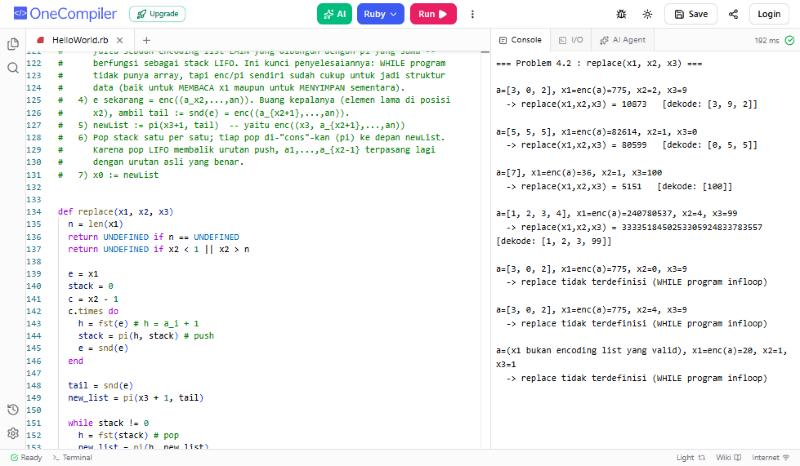
\includegraphics[width=\textwidth]{images/replace_execution.png}
    \caption{Kode Ruby \textit{replace} beserta hasil eksekusinya pada
    \textit{online Ruby compiler} (\url{https://onecompiler.com/ruby}).}
    \label{fig:replace}
\end{figure}
Ketujuh kasus cocok dengan definisi $replace$: hasil dekode selalu berupa
list asal dengan elemen ke-$x_2$ diganti $x_3$, dan tiga kasus terakhir
sengaja melanggar syarat $1\leq x_2\leq n$ (atau $x_1$ bukan $enc$ list
valid), semuanya benar dilaporkan tidak terdefinisi.

% =========================================================
% PROBLEM 4.3
% =========================================================

\section{Problem 4.3 -- \textit{isProg} adalah WHILE-Computable}

\subsection{Definisi Ulang Masalah dan Skema Encoding}
$isProg(x_1)=1$ jika $x_1$ adalah kode dari suatu GOTO program yang valid,
dan $isProg(x_1)=0$ jika bukan; fungsi ini \emph{total} (harus selalu
berhenti dan menjawab 0 atau 1). Skema encoding GOTO program yang dipakai
(Lect04 Slide 27--28): program $L_1{:}S_1;\dots;L_n{:}S_n$ dengan $k$
variabel input dan indeks variabel terbesar $m$ dikodekan sebagai
$$enc\big((k,\,m,\,enc(S_1),\dots,enc(S_n))\big),$$
dan setiap statement dikodekan menurut Tabel~\ref{tab:opcode}.

\begin{table}[H]
\centering
\begin{tabular}{ll}
\hline
Statement & Encoding \\ \hline
$x_i:=x_i+1$ & $enc((1,i))$ \\
$x_i:=x_i-1$ & $enc((2,i))$ \\
\texttt{GOTO} $L_j$ & $enc((3,j))$ \\
\texttt{IF} $x_i=0$ \texttt{THEN GOTO} $L_j$ & $enc((4,i,j))$ \\
\texttt{HALT} & $enc((5))$ \\ \hline
\end{tabular}
\caption{Skema encoding tiap jenis statement GOTO (Lect04 Slide 28).}
\label{tab:opcode}
\end{table}

\subsection{Keputusan Desain}
Spesifikasi soal tidak merinci beberapa hal secara eksplisit, sehingga
diambil keputusan desain berikut (dan diterapkan konsisten di WHILE program
maupun kode Ruby):
\begin{itemize}
    \item Indeks variabel $i$ pada opcode 1/2/4 boleh sembarang bilangan
    asli $\geq0$ (termasuk $x_0$), karena tata bahasa GOTO (Lect03 Slide
    22) tidak membatasi variabel mana yang boleh dipakai di suatu
    statement.
    \item Target lompatan $j$ pada opcode 3/4 \textbf{diwajibkan}
    $1\leq j\leq n$ (label tersebut harus benar-benar ada di program itu).
    Tanpa syarat ini, sembarang bilangan besar bisa "lolos" jadi target
    \texttt{GOTO} padahal labelnya tidak pernah ada -- yang secara intuitif
    bukan program yang well-formed.
    \item Tidak disyaratkan keberadaan/posisi \texttt{HALT} tertentu,
    karena tata bahasa (Lect03 Slide 21--22) hanya mensyaratkan tiap $S_i$
    berupa salah satu dari lima bentuk statement, tanpa aturan tambahan
    ihwal urutan atau keharusan \texttt{HALT}.
\end{itemize}

\subsection{Blok Bangunan yang Dipakai}
$isProg$ dibangun dari $isList$ (Slide 34--35, total), $len$ (Slide 36,
parsial), dan $elem$ (Slide 37, parsial) yang sudah terbukti WHILE-computable
di Lecture 4. Karena $isProg$ harus \emph{total} (tidak boleh pernah
infloop), setiap pemanggilan fungsi \emph{parsial} ($len$, $elem$) selalu
didahului pengecekan $isList$/batas panjang, persis pola yang dipakai
$elem$ sendiri terhadap $len$ di Slide 37.

\subsection{Program WHILE}
\begin{lstlisting}
# isProg(x1)
IF isList(x1) = 0 THEN
    x0 := 0
ELSE
    total := len(x1);              # aman: x1 sudah lolos isList
    IF total < 3 THEN               # perlu >=1 statement, plus k,m
        x0 := 0
    ELSE
        n   := total - 2;           # banyak statement
        bad := 0;
        t   := 0;
        LOOP n DO                   # t = 1..n (t dilacak lewat posisi elem)
            t := t + 1;
            IF bad = 0 THEN         # guard "early exit" ala WHILE (Lect02 S.34)
                stmt := elem(x1, t + 2);
                IF isList(stmt) = 0 THEN
                    bad := 1
                ELSE
                    slen := len(stmt);
                    op   := elem(stmt, 1);
                    valid := 0;
                    IF op = 1 OR op = 2 THEN
                        IF slen = 2 THEN valid := 1 END
                    END;
                    IF op = 3 THEN
                        IF slen = 2 THEN
                            j := elem(stmt, 2);
                            IF j >= 1 AND j <= n THEN valid := 1 END
                        END
                    END;
                    IF op = 4 THEN
                        IF slen = 3 THEN
                            j := elem(stmt, 3);
                            IF j >= 1 AND j <= n THEN valid := 1 END
                        END
                    END;
                    IF op = 5 THEN
                        IF slen = 1 THEN valid := 1 END
                    END;
                    IF valid = 0 THEN bad := 1 END
                END
            END
        END;
        IF bad = 0 THEN x0 := 1 ELSE x0 := 0 END
    END
END
\end{lstlisting}
(\texttt{LOOP n DO \dots END} dengan pencacah eksplisit $t$ adalah gula
sintaks yang sama seperti Problem 4.2 -- perulangan terhitung yang sudah
terbukti dapat diterjemahkan ke WHILE murni di Teorema 3.1 Lect03; \texttt{OR}/\texttt{AND}
adalah gula sintaks percabangan majemuk yang langsung tersusun dari
\texttt{IF}$\dots$\texttt{THEN} bersarang.)

\textbf{Kebenaran \& totalitas (sketsa).} Program di atas jelas selalu
berhenti (\emph{total}): pengecekan $isList(x_1)$ dan $total<3$ hanya
memanggil fungsi total, dan begitu keduanya lolos, $len(x_1)$ aman dipanggil
(tidak infloop). Loop utama berjalan tepat $n$ kali (terhitung, bukan
kondisional atas nilai yang bisa berubah tak terduga), dan di setiap
iterasi, $elem(x_1,t{+}2)$ selalu berada pada indeks valid
($3\leq t{+}2\leq n{+}2=total$), sehingga aman. Di dalam iterasi, $len(stmt)$
dan $elem(stmt,\cdot)$ hanya dipanggil setelah $isList(stmt)=1$ dipastikan,
dan indeks yang diminta ($1$; atau $2$ hanya jika $slen=2$; atau $3$ hanya
jika $slen=3$) selalu berada dalam batas -- jadi tidak pernah infloop.
Variabel \texttt{bad} menjadi $1$ tepat ketika ditemukan satu statement yang
strukturnya tidak cocok tabel opcode manapun (opcode di luar $1..5$, arity
salah, atau target lompatan di luar $[1,n]$); begitu \texttt{bad}=1, guard
\texttt{IF bad=0} membuat sisa iterasi tidak mengubah apa pun lagi (efeknya
sama seperti "berhenti memeriksa" begitu satu statement tidak valid
ditemukan). Akhirnya $x_0=1$ jika dan hanya jika \emph{semua} $n$ statement
valid -- persis definisi $isProg$. $\blacksquare$

\subsection{Implementasi Ruby \& Hasil Eksekusi}
Implementasi lengkap ada pada berkas \texttt{is\_prog.rb}. Inti fungsinya:
\begin{lstlisting}
def is_prog(x1)
  return 0 if is_list(x1).zero?

  total = len(x1)
  return 0 if total < 3

  n = total - 2
  bad = 0

  (1..n).each do |t|
    next unless bad.zero?

    stmt = elem(x1, t + 2)
    if is_list(stmt).zero?
      bad = 1
      next
    end

    slen = len(stmt)
    op = elem(stmt, 1)

    valid =
      case op
      when 1, 2 then slen == 2
      when 3
        slen == 2 && (j = elem(stmt, 2)) && j >= 1 && j <= n
      when 4
        slen == 3 && (j = elem(stmt, 3)) && j >= 1 && j <= n
      when 5 then slen == 1
      else false
      end

    bad = 1 unless valid
  end

  bad.zero? ? 1 : 0
end
\end{lstlisting}

Hasil eksekusi kode (gabungan \texttt{enc\_helpers.rb} dan
\texttt{is\_prog.rb}) pada \textit{online Ruby compiler} ditunjukkan pada
Gambar~\ref{fig:isprog-a} dan Gambar~\ref{fig:isprog-b} (keluaran konsol
cukup panjang sehingga dibagi dua tangkapan layar dari eksekusi yang sama),
termasuk verifikasi ulang terhadap contoh program \texttt{add} 9-baris
persis dari Lect03/Lect04.
\begin{figure}[H]
    \centering
    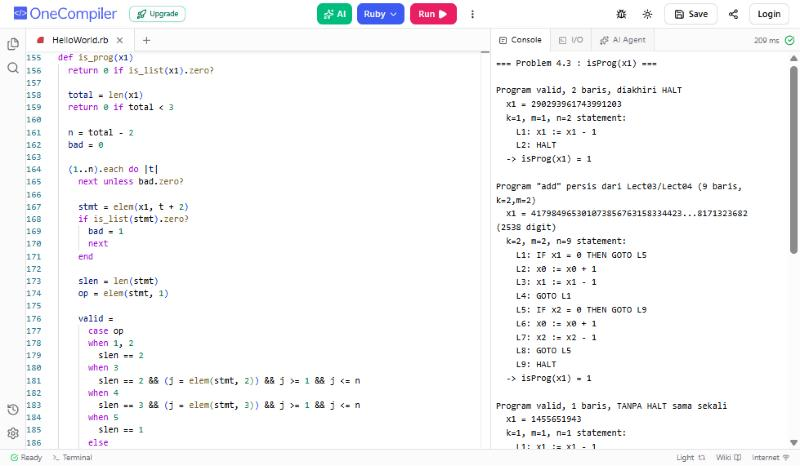
\includegraphics[width=\textwidth]{images/isprog_execution_a.png}
    \caption{Kode Ruby \textit{isProg} dan keluaran konsol bagian pertama
    (program valid, termasuk contoh \texttt{add}), dijalankan pada
    \textit{online Ruby compiler} (\url{https://onecompiler.com/ruby}).}
    \label{fig:isprog-a}
\end{figure}
\begin{figure}[H]
    \centering
    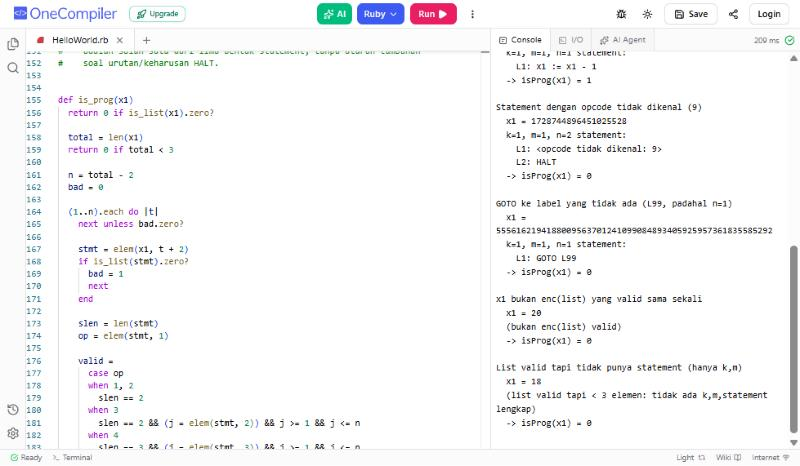
\includegraphics[width=\textwidth]{images/isprog_execution_b.png}
    \caption{Keluaran konsol bagian kedua dari eksekusi yang sama (kasus
    yang bukan kode GOTO program).}
    \label{fig:isprog-b}
\end{figure}
Tujuh kasus di atas mencakup: dua program valid (dengan dan tanpa
\texttt{HALT}), rekonstruksi persis contoh \texttt{add} dari kelas
(membuktikan encoding \& decoding konsisten bolak-balik pada kasus nyata
yang jauh lebih besar, $2538$ digit), serta empat cara berbeda suatu
bilangan bisa gagal jadi kode GOTO program (opcode tak dikenal, target
lompatan di luar batas, bukan $enc$ list sama sekali, dan list valid tapi
tidak berisi statement) -- semuanya dijawab \texttt{isProg}=$0$ sesuai
definisi.

% =========================================================
% PRANALA KODE
% =========================================================

\section{Pranala Kode}
Seluruh kode Ruby (\texttt{enc\_helpers.rb}, \texttt{replace.rb},
\texttt{is\_prog.rb}) beserta hasil \textit{running}-nya dapat diakses di
pranala repositori GitHub berikut:
\begin{center}
    \url{https://github.com/khalilullahalfaath/assignment-4-tekkom-encoding}
\end{center}

\end{document}
